\subsection{Regelmäßiges Ausrichten der Wände (Janneke)}

Da die Änderung des Referenzscan-Updates, um einen Drift des Scans über die Zeit abzumildern, nicht ganz den gewünschten Effekt hatte und eher zu mehr Problemen geführt hat, haben wir versucht das Problem anders zu lösen. Bei den Tests fällt auf, dass der Drift der Rotation ein größeres Problem zu sein scheint, als der Translations-Drift. Da wir nur ganz am Anfang den initialen Scan auf die Hauptachsen ausrichten und dann darauf vertrauen, dass alle weiteren Scans durch die Rotationskorrektur richtig ausgerichtet werden, liegt es nahe diesen Schritt auch in der Schleife ab und zu durchzuführen. Dies sollte den Drift über die Zeit gut kompensieren können.

Hierbei ist es wichtig, dass das Maximum welches im Histogramm gefunden wird mit der Achse korrespondiert mit der es auch zuvor korrespondiert hat, da je nach Position und Orientierung unterschiedliche Wände im Histogramm besonders stark erkennbar sind. Hierfür nehmen wir an, dass wir gerade Wände, bzw. Linien haben, die 90 Grad aufeinander stehen. Da das Verfahren sowieso auf dieser Annahme beruht schränken wir es damit nicht weiter ein. Bei einem Histogramm das auf einem, auf die Hauptachsen ausgerichteten, Scan berechnet wurde, sollen die Peaks nun also auf 0, 90, 180, 270 oder 360 Grad liegen. Wir berechnen nun also die Rotation die das Maximum im Winkelhistogramm auf einen dieser Werte schiebt und wenden diese zusätzlich auf den Scan an, bevor wir diesen in die Karte eintragen. Die Rotation muss natürlich auch auf den globalen Rotationsoffset addiert werden, damit spätere Scans auf diesen neuen Scan ausgerichtet werden.

Abbildung~\ref{fig:AchsenAlign_4min}-\ref{fig:AchsenAlign_10min} stellen unser Verfahren mit und ohne Ausrichtungs-Update zu unterschiedlichen Fahrzeiten gegenüber. Während die Karten bei einer Fahrzeit von einer Minute noch recht ähnlich aussehen ist bei einer Fahrzeit von 4 Minuten schon gut zu erkennen, dass die Karte mit Ausrichtungs-Update (Abbildung~\ref{fig:AchsenAlign_4min} links) weniger dicke Wände hat als die Karte ohne Ausrichtungs-Update (Abbildung~\ref{fig:AchsenAlign_4min} rechts). Des Weiteren ist gut zu erkennen, dass sich die Karten mit Ausrichtungs-Update zwischen einer Fahrzeit von 7 (Abbildung~\ref{fig:AchsenAlign_7min} links) und 10 (Abbildung~\ref{fig:AchsenAlign_10min} links) Minuten kaum verändern, während bei den Karten ohne Ausrichtungs-Update erkennbar ist, dass sich die Karte immer weiter verschlechtert (Abbildung~\ref{fig:AchsenAlign_7min} rechts \& \ref{fig:AchsenAlign_10min} rechts)  

Die neue Ausrichtung der Scans soll nun aber nicht in jedem Schritt passieren, sondern nur über die Zeit den Drift verhindern. Daher haben wir verschiedene Schrittgrößen angefangen bei jedem 10. Karten-Update ausprobiert. Dabei haben wir festgestellt, dass ein Ausrichtungs-Update alle 5 Karten-Updates ein guter Wert ist.

\begin{figure}
	\centering
	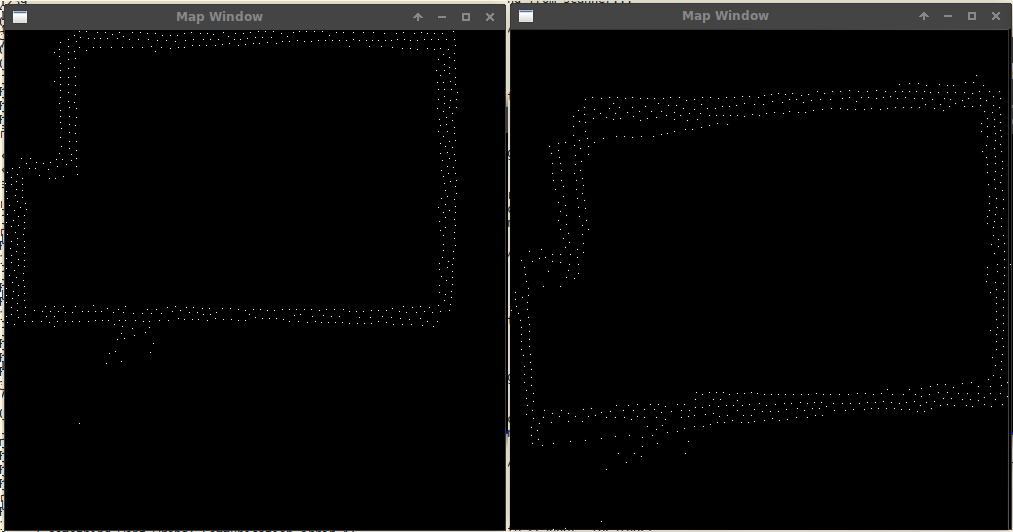
\includegraphics[width=14cm]{mitAchsenAlignLINKS_ohneRECHTS_4min}
	\caption{Links: Karte mit Ausrichtungs-Update alle 10 Karten-Update Schritte, 4 Minuten Fahrzeit; Rechts: Karte ohne Ausrichtungs-Updates, 4 Minuten Fahrzeit}
	\label{fig:AchsenAlign_4min}
\end{figure}

\begin{figure}
	\centering
	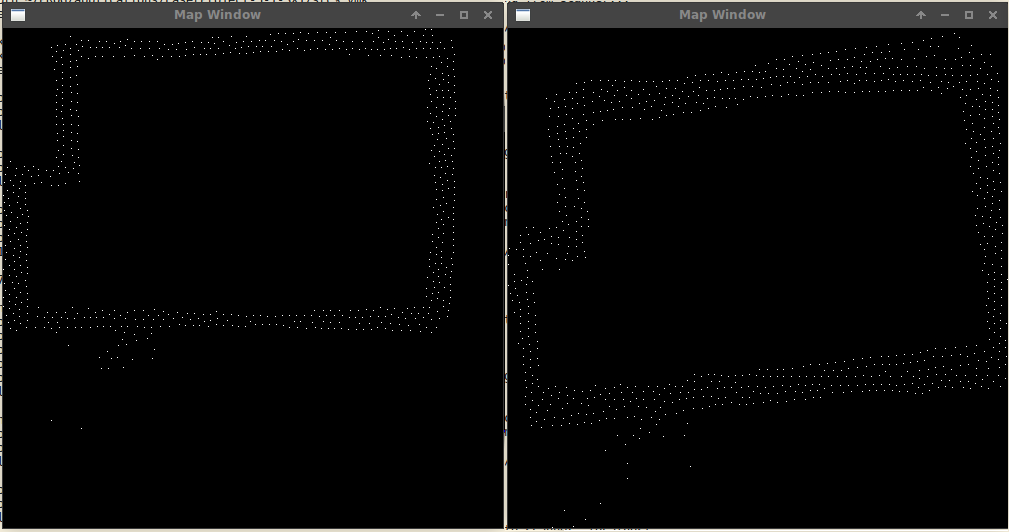
\includegraphics[width=14cm]{mitAchsenAlignLINKS_ohneRECHTS_7min}
	\caption{Links: Karte mit Ausrichtungs-Update alle 10 Karten-Update Schritte, 7 Minuten Fahrzeit; Rechts: Karte ohne Ausrichtungs-Updates, 7 Minuten Fahrzeit}
	\label{fig:AchsenAlign_7min}
\end{figure}

\begin{figure}
	\centering
	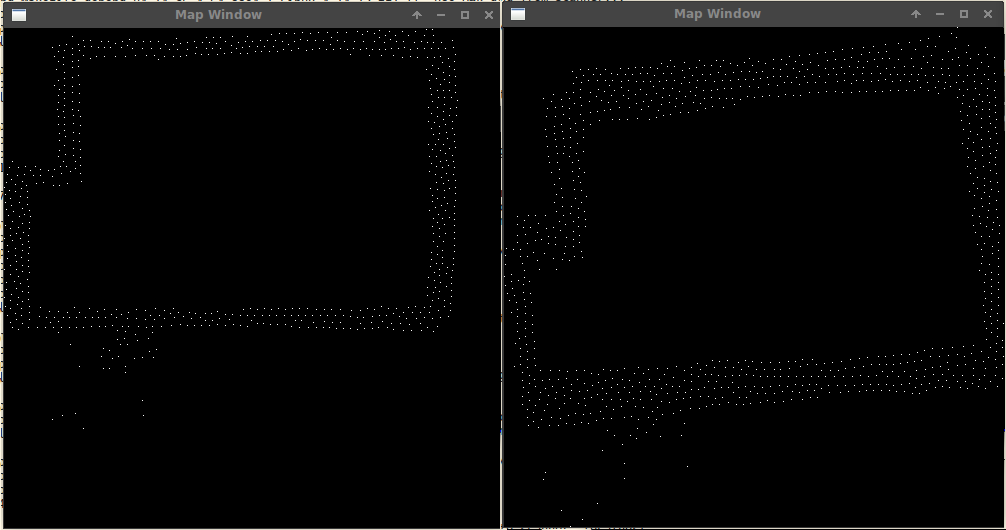
\includegraphics[width=14cm]{mitAchsenAlignLINKS_ohneRECHTS_10min}
	\caption{Links: Karte mit Ausrichtungs-Update alle 10 Karten-Update Schritte, 10 Minuten Fahrzeit; Rechts: Karte ohne Ausrichtungs-Updates, 10 Minuten Fahrzeit}
	\label{fig:AchsenAlign_10min}
\end{figure}

\newpage